\documentclass{ieeetj}

\usepackage{amsmath}
\usepackage{amssymb}
\usepackage{booktabs}
\usepackage{cite}
\usepackage{graphicx}
\usepackage{placeins}
\usepackage{tabularx}
\usepackage{url}
\usepackage{xcolor}
\usepackage{etoolbox}
\AtBeginDocument{\definecolor{tmlcncolor}{cmyk}{0.93,0.59,0.15,0.02}\definecolor{NavyBlue}{RGB}{0,86,125}}
\graphicspath{{figures/}}
% Official IEEE OJ-CS template (selector publication 210, template 477).
% Publisher-assigned branding, dates, DOI, and volume are not invented.
\def\OJlogo{}
\def\seclogo{}
\makeatletter
\let\@revised\@empty
\patchcmd{\@maketitle}{\fi.\space}{\fi\space}{}{}
\def\ps@submission{\def\@oddhead{}\def\@evenhead{}%
  \def\@oddfoot{\hfil\thepage\hfil}\let\@evenfoot\@oddfoot}
\makeatother

\title{Regime-Adaptive Risk-Aware MPPI Control for Force-Aware Robotic Wiping with Temporal-Difference World Models}

\author{Zhiheng Li\textsuperscript{1}}
\affil{Independent Researcher, Shanghai, China}
\corresp{Corresponding author: Zhiheng Li (email: LLzhiheng@outlook.com).}

\begin{document}
\markboth{}{Li}

\begin{abstract}
Force-aware wiping requires contact acquisition, force regulation, transient
control, and surface progression. We introduce regime-adaptive risk-aware
model-predictive path integral (MPPI) planning for direct temporal-difference
model-predictive control (TD-MPC2) wiping. The method retains requested force
in latent dynamics and adapts planning costs and computation from causal
contact regimes and learned next-force predictions. Across 270 paired
factor-separated evaluations, it raises compound pass from 85/135 to 100/135
(+11.11 percentage points; block- and seed-aware 95\% interval [3.70, 18.52]),
reduces mean relative error by 1.83 points, and uses 8.0 fewer samples and
25.7~ms less median planning time. Task completion remains 132/135 versus
133/135, and both planners record two samples above 15~N. A 375-run one-factor
panel identifies force bias, 50-ms delay, and registered-normal error as
distinct sensitivities. In a zero-shot MuJoCo stress test, all 30 flat and
inclined evaluations retain the compound outcome, whereas none of 15 weakly
curved evaluations does. Regime adaptation therefore improves the
tracking--computation trade-off in simulation, while curved contact remains
the principal portability boundary.
% Insert the stable anonymous artifact URL here after double-blind deposition.
\end{abstract}


\begin{IEEEkeywords}
contact-rich manipulation, cross-simulator transfer, force-aware control,
model-predictive path integral control, robotic wiping, TD-MPC2
\end{IEEEkeywords}
\maketitle
\pagestyle{submission}
\thispagestyle{submission}

\section{Introduction}
\label{sec:introduction}

Robotic wiping is a contact-rich control problem in which geometric progress
and force regulation must succeed together. The tool must first acquire the
surface, approach a requested load without a large transient, maintain useful
contact during motion, and recover when contact is lost. These phases place
different demands on a controller. Contact acquisition rewards decisive
inward motion, stable tracking rewards accurate force regulation, and rapid
force growth calls for conservative action. A planning objective and sampling
budget that remain fixed throughout an episode need not serve all three
requirements equally well.

Temporal-difference model-predictive control (TD-MPC2) offers a natural basis
for this problem: a learned actor provides a policy prior, while a latent
world model evaluates action sequences online
\cite{hansen2024tdmpc2,williams2018information}. Earlier ForceWipe experiments
showed that behaviour-cloning (BC)-assisted TD-MPC2 could complete controlled
first-pass wiping directly at 5, 8, and 12~N. They also exposed three limits.
First, a hard measured-force threshold routed between the actor and planner
without adapting the planning objective itself. Second, the 12~N tier retained
a systematic negative force bias. Third, the matched actor-only comparison
did not resolve a general performance benefit from online planning despite a
clear computation cost. These observations motivate a method that changes
what the planner optimizes and how much it searches, rather than merely
changing when planning is enabled.

We introduce regime-adaptive risk-aware MPPI (RA-RMPPI), a unified planner for
direct TD-MPC2 wiping. The requested force is encoded by a dedicated condition
branch and retained through imagined latent transitions. Learned next-force
predictions provide a causal risk signal. Smooth causal memberships represent
acquisition, approach, tracking, recovery, and transient risk. They
continuously adjust contact, tracking, transient, and actor-anchor costs
together with the MPPI sample count, optimization
iterations, and exploration scale. The actor remains the proposal
distribution in every regime; the historical hard actor--planner switch is
removed.

The empirical design separates method selection from evaluation. Five
unfiltered seeds share the same data and update budget. A four-arm ablation
isolates adaptive objectives and adaptive computation, while additional
ablations examine behaviour-cloning strength, transient-risk representation,
and the historical routing threshold. The method is then evaluated on new
factor-separated shifts in surface geometry and contact dynamics, avoiding
the path--surface--tool confounding of the earlier combined
out-of-distribution (OOD) blocks. Across 270 paired evaluations, the complete
method raises compound pass from 85/135 to
100/135 while using fewer planning samples and less host planning time. The
gain is concentrated in force regulation: task completion and sampled force
violations do not improve, and the cylindrical 12~N condition remains a
failure boundary. A zero-shot MuJoCo stress test sharpens that boundary: all
30 flat and inclined evaluations achieve the compound outcome, whereas none of
the 15 cylindrical evaluations does.

The paper makes three contributions. First, it presents a force-conditioned
latent dynamics construction that preserves the requested force during
multi-step imagination. Second, it develops a regime-adaptive risk objective
and compute schedule that unifies acquisition, tracking, and recovery without
a discrete actor--planner router. Third, it provides matched component and
training ablations, including negative evidence for a more elaborate
transient-envelope representation, together with factor-separated and
cross-engine simulation evaluation. The resulting evidence identifies a
statistically resolved tracking--computation improvement while preserving the
method's unresolved curvature and force-tail limits.

\section{Related Work}
\label{sec:related_work}

\subsection{Robot Wiping and Surface Interaction}

Surface processing couples geometric coverage with sustained contact.
Probabilistic Surface Interaction Primitives (ProSIP) conditions compliant
motions on tool-centre-point (TCP) pose, surface geometry, and context
\cite{unger2024prosip}. Adaptive Wiping combines few-shot imitation,
force--torque feedback, and pre-trained object representations
\cite{tsuji2025adaptivewiping}. Liu \emph{et al.} study quality-critical wiping
over randomised curvatures, frictions, and waypoints using a visual-language
curriculum; their 20~Hz pose policy operates through an operational-space
controller around a 60~N force target~\cite{liu2025wipingvlm}. We examine direct
learned Cartesian displacements at 5, 8, and 12~N.

Variable Impedance Control in End-Effector Space (VICES) uses variable
impedance as a reinforcement-learning (RL) action space, including for wiping
\cite{martinmartin2019vices}. Beltran-Hernandez \emph{et al.} combine RL with
parallel position--force or admittance control and a real-robot fail-safe
\cite{beltranhernandez2020force}. Zhu \emph{et al.} couple an image-based
equilibrium-point/impedance policy with faster contact-aware control
\cite{zhu2022contactsafe}. Force-Guided Exploration for Robust Contact-Rich
Manipulation under Uncertainty (FORGE) conditions assembly policies on a
maximum allowable force and uses dynamics randomisation for hardware transfer
\cite{noseworthy2025forge}. These approaches structure learned contact through
the action space or execution layer. Our matched comparison uses a common
Cartesian-delta interface for TD-MPC2 and proximal policy optimisation (PPO),
with adaptive admittance as a separate reference.

Curved-surface methods also control tool orientation. Armesto \emph{et al.}
transfer planar wiping to unknown curves by estimating the contact constraint
and aligning the tool from force/torque feedback
\cite{armesto2018constraintaware}. Li \emph{et al.} estimate pose deviation,
lift a planar path onto an unknown workpiece, and close a normal-force loop
\cite{li2023unknownsurface}. Our registered frame supplies a local normal, but
Eq.~\eqref{eq:task_frame_map} controls translation only. Tool posture is not a
policy action, a distinction relevant to the observed curved-contact boundary.

\subsection{Force Control and Contact Simulation}

Hybrid position--force control separates directional objectives
\cite{raibert1981hybrid}; impedance and admittance regulate complementary
motion--force relations~\cite{hogan1985impedance,ott2010unified}. Our adaptive
admittance baseline shares the time-causal observation and actuator action box.
Force-feedback model-predictive control (MPC) offers another approach:
Kleff \emph{et al.} incorporate measured force/torque through robot-actuation
dynamics~\cite{kleff2022forcefeedbackmpc}, while Jordana \emph{et al.} estimate
force-model discrepancy online without an explicit contact-force evolution
model~\cite{jordana2024forcefeedbackmpc}. Our controller instead learns latent
dynamics conditioned on scalar normal force and issues displacements without
a separate force-control layer.

Runtime shields modify policy proposals~\cite{alshiekh2018shielding}, and
control barrier functions can enforce forward-invariance conditions
\cite{ames2019cbf,cheng2019rlcbf}. Here, learned actions execute without an
external shield or force-dependent post-processing. Sampled force exceedances
are therefore empirical observations for a specified numerical configuration,
not formal invariance guarantees. Contact models, relaxations, and solvers can
produce different application-level behaviour~\cite{lelidec2024contact};
Sec.~\ref{sec:credibility_audit} tests the sensitivity of our force-tail claims.

\subsection{Direct Model-Based Reinforcement Learning}

Temporal-difference model-predictive control (TD-MPC) and TD-MPC2 combine
latent dynamics, value prediction, and online planning
\cite{hansen2022tdmpc,hansen2024tdmpc2}. We retain actor-guided MPPI, replacing
the earlier force-threshold router with continuous causal memberships that
adapt planning costs and search budget. A same-checkpoint fixed-planner
ablation isolates this adaptation from the learned actor and world model.
PPO~\cite{schulman2017ppo} provides a direct model-free comparator, with its
training budget and hyperparameters examined separately.

Structured alternatives include residual RL around a conventional controller
\cite{johannink2019residual}, parameterised action primitives and Manipulation
Primitive-augmented Reinforcement Learning (MAPLE)
\cite{dalal2021raps,nasiriany2022maple}, and impedance primitive-augmented
hierarchical reinforcement learning (IMP-HRL)~\cite{tahmaz2025imphrl}. Our
study instead tests regime-adaptive planning within direct actor/world-model
control, using controlled variation, weak-curvature transfer, and
claim-specific numerical auditing.

% Requires: \usepackage{amsmath,amssymb,booktabs,tabularx}
\providecommand{\Ftgt}{F^{\star}}
\providecommand{\Fmin}{F_{\min}}
\providecommand{\Fmax}{F_{\max}}
\providecommand{\Faud}{F^{\mathrm{aud}}}
\providecommand{\ind}{\mathbb{I}}

\section{Simulation Task and Evaluation Suite}
\label{sec:benchmark}

We use ForceWipe as a controlled simulation testbed for direct first-pass
wiping. A successful evaluation must traverse the path, maintain useful
contact, track the target normal force, and avoid recorded force-limit
exceedances. The test cases vary path geometry, surface orientation, tool
profile, contact parameters, disturbances, and weak surface curvature. The
resulting suites define controlled and transfer conditions for the same direct
action interface.

\subsection{Direct First-Pass Task}
\label{subsec:task}

A seven-degree-of-freedom Franka Emika Panda manipulates a wiping tool in
ManiSkill3 with the PhysX central processing unit (CPU)
backend~\cite{xiang2020sapien,c_maniskill}.
Physics and control advance together at $100$~Hz. At each step, the local task
frame is formed by the path tangent $\mathbf{t}_t$, outward surface normal
$\mathbf{n}_t$, and cross-track axis
$\mathbf{c}_t=\mathbf{n}_t\times\mathbf{t}_t$. The controller outputs
\begin{equation}
\mathbf{a}_t=
\begin{bmatrix}a_t^{\parallel}&a_t^{\perp}&a_t^{n}\end{bmatrix}^{\!\top}
\in[-1,1]^3,
\label{eq:direct_action}
\end{equation}
where the components request along-path, cross-track, and inward-normal
displacements. The fixed, force-independent actuator map is
\begin{equation}
\Delta\mathbf{x}_t=
(0.50\,\mathrm{mm})a_t^{\parallel}\mathbf{t}_t
+(0.25\,\mathrm{mm})a_t^{\perp}\mathbf{c}_t
-(0.50\,\mathrm{mm})a_t^{n}\mathbf{n}_t.
\label{eq:task_frame_map}
\end{equation}
Post-policy processing consists exclusively of action-box clipping and a
force-independent coordinate transform in \eqref{eq:task_frame_map}.

The tangent and normal are evaluated from the registered nominal path and
surface model at the simulator-state tool pose. They are not inferred from a
camera, force sensor, or the TD-MPC2 latent state. Consequently, ``direct'' in
this study denotes the absence of a separate force-control or shielding layer;
it does not denote model-free geometric perception. This registered-frame
assumption is shared by all compared methods.

At decision step $t$, $F_t$ denotes the force supplied to the causal
observation before $\mathbf{a}_t$ is selected. We reserve $\Faud_t$ for the
native force read back after the corresponding physics step and attached to
that transition for evaluation. The target normal force is
$\Ftgt\in\{5,8,12\}$~N. The online contact indicator uses
$F_t\geq\Fmin=3$~N, whereas evaluation metrics use the post-step contact set
$\Faud_t\geq\Fmin$ defined in Sec.~\ref{subsec:metrics}. A strict sampled violation is
$\Faud_t>\Fmax=15$~N. The statement ``zero
violations'' therefore means that no recorded $100$-Hz sample exceeded
$15$~N. All force-limit results use this native sampled definition.
The three force targets, the 3-N contact threshold, and the 15-N sampled
limit form the frozen operating contract of this simulation task. They are
used identically by every method and were fixed before the controlled and
factor-separated evaluations; they are not presented as general robot or
human-contact safety standards.

Each path is divided into 20 normalized progress bins. A bin is marked
complete once it has accumulated at least two samples satisfying
$\Fmin\leq\Faud_t\leq\Fmax$, corresponding to $20$~ms at the simulator
rate. A task pass requires a single first-pass lifecycle to terminate with
all 20 bins complete and progress $s\geq0.98$. Re-wiping is disabled in all
three evaluation suites. The dose endpoint is synthetic contact
coverage and serves as the completion proxy.

\subsection{Controlled Evaluation Blocks}
\label{subsec:controlled_suite}

The initial and held-out controlled suites use three
surface orientations (flat, $5^{\circ}$ incline,
and $10^{\circ}$ incline), five path families (line, diagonal, arc,
S-curve, and polyline), and three tool profiles (wide-soft, narrow-soft, and
wide-hard). Their synthetic residual fields comprise single-blob, islands,
edge-dense, stripe or multimodal, and Gaussian-random-field patterns. These
factors are assembled into prespecified blocks rather than sampled as an
independent factorial design.

The five initial blocks Q0--Q4 use the nominal contact plant and
no exogenous disturbance. They vary path length between approximately
$0.156$ and $0.166$~m while changing geometry, tool, and residual field by
block. The ten previously unused held-out blocks C0--C9 form two disjoint
groups. C0--C4 repeat the five path families on a nominal plant. C5--C9
pair the same roster positions with randomised path length, friction,
support stiffness, effective mass, damping, and restitution. Their frozen
definitions also label designated blocks with lateral or normal impulses,
reference noise, and delayed sensor noise. A later binding audit established
the physical impulse call chain but did not establish that the declared
reference-noise and sensor-noise signals reached the direct controller's
learner-visible force path. We therefore make no robustness claim for those
two declared noise conditions. Because several verified attributes change
jointly, grouped path, surface, tool, residual, and plant summaries quantify
block-level transfer rather than single-factor effects.

\subsection{Weak-Curvature Out-of-Distribution Blocks}
\label{subsec:weak_curvature_suite}

The matched OOD study contains six previously unused, prespecified blocks
F0--F5. All surfaces are static cylinders with radii $1.2$--$1.8$~m. Its paths
are arc, S-curve, or polyline trajectories with lengths $0.13$--$0.205$~m.
Across the six blocks, the study includes all three tool profiles, six
residual families, randomised friction and contact plant parameters, and
predefined disturbance labels. Physical lateral and normal impulse call chains
are present in their designated blocks; the declared reference-noise and
sensor-noise/latency effects are excluded from the evidence claims because
their runtime binding was not established. Table~\ref{tab:evaluation_suites}
summarizes the evaluation stages.

\begin{table*}[t]
\centering
\caption{Prespecified simulation suites. Evaluation totals are Cartesian
products of blocks, force targets, and method replicates; blocks are the
environment units. For the deployment-gap panel, 375+45 denotes new stress
evaluations plus reused nominal evaluations.}
\label{tab:evaluation_suites}
\small
\setlength{\tabcolsep}{4.5pt}
\begin{tabular}{@{}lccccp{6.1cm}@{}}
\toprule
Stage & Blocks & Targets & Replicates & Evaluations & Main variation \\
\midrule
Controlled evaluation
& 5 & 3 & 5 checkpoints & 75
& Five paths; flat/$5^{\circ}$/$10^{\circ}$ surfaces; three tools; nominal plant \\
Held-out controlled evaluation
& 10 & 3 & 5 checkpoints & 150
& Five nominal multipath blocks plus five randomised-plant/disturbance blocks \\
Matched weak-curvature OOD
& 6 & 3 & method dependent & 288
& Static weak-curvature cylinders, three paths, three tools, randomised plant, and disturbances \\
Numerical sentinel panel
& 4 & 1 & one checkpoint & 36
& Four 12~N OOD baseline reproductions plus 32 solver, contact-offset, mesh, and interaction cells \\
Deployment-gap stress
& 3 & 3 & 5 checkpoints & 375+45
& Learner-visible force noise/bias, delay, TCP-position error, and registered-frame normal error \\
\bottomrule
\end{tabular}
\end{table*}

The controlled and weak-curvature suites are reported separately to preserve
their deliberately different scenario distributions.

\subsection{Evaluation Metrics and Success Criteria}
\label{subsec:metrics}

Force tracking is computed over the finite contact set
\begin{equation}
\mathcal{T}_{c}=\{t\mid \Faud_t\geq3~\mathrm{N}\}.
\end{equation}
If $\mathcal{T}_{c}$ is empty, the force-tracking metrics are undefined and
the evaluation fails the tracking criterion. For a nonempty contact set, we
report mean relative error (MRE), root-mean-square error (RMSE), and normalized
root-mean-square error (NRMSE):
\begin{align}
\overline F_c
&=\frac{1}{|\mathcal{T}_{c}|}
\sum_{t\in\mathcal{T}_{c}}\Faud_t,\nonumber\\
b_F&=\overline F_c-\Ftgt,\qquad
\mathrm{MRE}=\frac{|b_F|}{\Ftgt},\nonumber\\
\mathrm{RMSE}
&=\sqrt{\frac{1}{|\mathcal{T}_{c}|}
\sum_{t\in\mathcal{T}_{c}}(\Faud_t-\Ftgt)^2},\nonumber\\
\mathrm{NRMSE}&=\frac{\mathrm{RMSE}}{\Ftgt}.
\label{eq:force_metrics}
\end{align}
Tracking is considered successful when
$\mathrm{MRE}\leq0.15$ and $\mathrm{NRMSE}\leq0.20$. Signed bias is
retained so systematic under-tracking remains visible even when both
tolerances are met. These two tolerances are likewise study-defined acceptance
criteria frozen with the evaluation protocol, rather than thresholds inferred
from the reported trials.

The force evaluation records episode peak force, peak overshoot
$\max(\max_t\Faud_t-\Ftgt,0)$, peak-force mean, 95th percentile (P95), and
maximum, and sample counts
above $14.5$ and $15$~N. The $14.5$~N count is descriptive headroom; the
sampled-force-limit criterion requires zero samples above $15$~N. Contact metrics
include contact fraction and, after first contact, the number, total duration,
and maximum duration of maximal consecutive intervals below $3$~N.
Force-tail quantities describe the frozen numerical configuration in which
they were observed. Section~\ref{sec:credibility_audit} separately tests their
sensitivity to selected simulator settings.

An evaluation satisfies deployment integrity when every trace confirms
direct-action interface compliance: the selected learned branch issued the
executed action, followed by the fixed map in \eqref{eq:task_frame_map}. A
\emph{compound pass} is the intersection of task completion, tracking,
sampled-force-limit compliance, and deployment integrity. Nonfinite force or
an empty contact set counts as an evaluation failure. Planning time and the
actor/MPPI action fractions are descriptive computational metrics.

\subsection{Scope of the Suite}
\label{subsec:scope}

The blocks are fixed conditions, with each block defining an
environment unit. Replicated checkpoint--block--target trials increase the
precision of within-design comparisons. The suite characterizes direct
force-aware wiping under controlled variation and weak-curvature transfer;
Sec.~\ref{sec:discussion} defines the corresponding deployment scope.

\section{Regime-Adaptive Risk-Aware World-Model Control}
\label{sec:ra_method}

The proposed controller retains the learned latent dynamics, force predictor,
and policy prior of TD-MPC2. Its contribution is
to couple these components through a causal, state-dependent planning
objective rather than a fixed force threshold. The policy prior proposes
candidate actions in every contact regime. A single model-predictive path
integral (MPPI) planner then changes its objective and computational budget
according to the current force state and the model's predicted transient-risk
estimate. No classical force controller, post-hoc action projection, or
evaluation-time teacher is introduced.
Figure~\ref{fig:ra_rmppi_architecture} summarizes the resulting data flow.

\begin{figure*}[t]
\centering
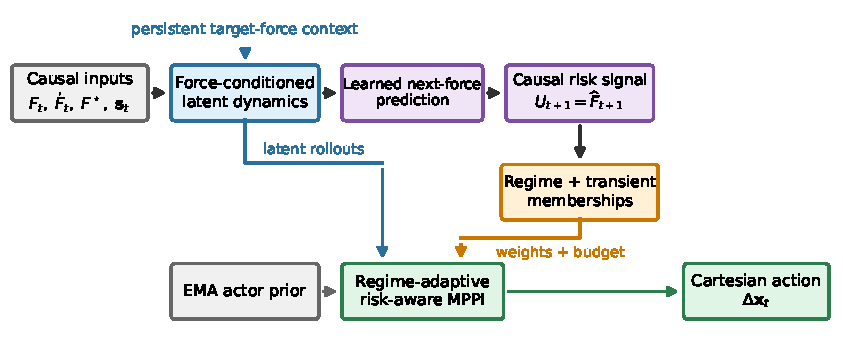
\includegraphics[width=0.96\textwidth]{figures/ra_rmppi_architecture.pdf}
\caption{Force-conditioned regime-adaptive risk-aware MPPI architecture.}
\label{fig:ra_rmppi_architecture}
\end{figure*}

Let $F_t$, $F^\star$, and $\dot F_t$ denote measured force, requested force,
and measured force rate. Unlike an observation-only target input, the requested
force is encoded by a dedicated condition branch
$\mathbf c_t=e_\theta(F^\star)$. The latent state concatenates a base state and
this condition, $\mathbf z_t=[h_\theta(\mathbf o_t);\mathbf c_t]$, and the
imagined transition is
\begin{equation}
\mathbf z_{t+1}=
\left[f_\theta(\mathbf z_t,\mathbf a_t,\mathbf c_t);\mathbf c_t\right].
\label{eq:force_conditioned_dynamics}
\end{equation}
The copied condition prevents the requested force from being diluted over a
multi-step rollout while the learned base dynamics remain action dependent.
For candidate action $\mathbf a_t$, the selected world-model risk
representation is the predicted next force
\begin{equation}
U_{t+1}=\widehat F_{t+1}.
\label{eq:ra_upper_prediction}
\end{equation}
During an $H$-step imagined rollout, this head is evaluated after every
latent transition, producing the causal transient forecast
$\widehat{\mathbf F}_{t+1:t+H}$ used by the tracking and transient costs.
This choice follows a matched development ablation against a learned
transient-envelope point prediction and a target-calibrated alternative;
neither alternative improved the prespecified outcomes.

Smooth causal memberships
\begin{equation}
\boldsymbol\pi_t=
[\pi_t^{\mathrm{acq}},\pi_t^{\mathrm{app}},
\pi_t^{\mathrm{track}},\pi_t^{\mathrm{rec}}]
\end{equation}
distinguish initial contact
acquisition, approach to the force target, stable tracking, and recovery after
contact loss. A fifth, overlapping membership $\pi_t^{\mathrm{tr}}$ measures
transient risk from $U_{t+1}$ and positive force rate. These memberships depend
only on $(F_t,F^\star,\dot F_t,U_{t+1})$ and episode-level contact history.
They replace the previous hard switch at $0.85F^\star$.

Let $r_t=\max(F_t,0)/F^\star$, let
$\sigma(x)=(1+\exp(-x))^{-1}$, and let $h_t\in\{0,1\}$ record whether
contact has occurred earlier in the episode. The unnormalized phase scores are
\begin{align}
\widetilde\pi_t^{\mathrm{acq}}
  &=(1-h_t)\sigma\!\left(10\frac{3-F_t}{F^\star}\right),\\
\widetilde\pi_t^{\mathrm{rec}}
  &=h_t\sigma\!\left(10(0.65-r_t)\right),\\
\widetilde\pi_t^{\mathrm{app}}
  &=\sigma\!\left(10(0.90-r_t)\right),\\
\widetilde\pi_t^{\mathrm{track}}
  &=\exp\!\left[-\frac{1}{2}\left(\frac{r_t-1}{0.15}\right)^2\right].
\end{align}
Normalizing these four scores gives $\boldsymbol\pi_t$. Transient membership
overlaps the phase simplex:
\begin{align}
\pi_t^{\mathrm{tr}}=1
&-\left[1-\sigma\!\left(10\frac{U_{t+1}-14.5}{0.5}\right)\right]\nonumber\\
&\quad\times\left[1-\sigma\!\left(10\left(\frac{\max(\dot F_t,0)}{80}-1\right)\right)\right].
\label{eq:transient_membership}
\end{align}
Forces are in newtons and force rate is in newtons per second. The membership
is therefore high when either the predicted next force approaches the force
limit or measured force rises rapidly.

The force thresholds in these memberships inherit the task contract in
Sec.~\ref{subsec:task}. The remaining ratios, bandwidth, sigmoid gain, and
force-rate scale are development-fixed design parameters: they create smooth,
overlapping transitions rather than learned decision boundaries. They were
held fixed before the nine-block evaluation, and no coefficient in
Eqs.~\eqref{eq:transient_membership}--\eqref{eq:adaptive_weights} was fitted on
those final blocks.

For a candidate sequence $\mathbf a_{t:t+H-1}$, the planner maximizes
\begin{align}
J_t={}&J_{\mathrm{task}}
-\lambda_c(\boldsymbol\pi_t)J_{\mathrm{contact}}
-\lambda_f(\boldsymbol\pi_t)J_{\mathrm{tracking}}\nonumber\\
&-\lambda_r(\boldsymbol\pi_t)J_{\mathrm{transient}}
-\lambda_a(\boldsymbol\pi_t)J_{\mathrm{anchor}},
\label{eq:ra_objective}
\end{align}
where $J_{\mathrm{tracking}}$ penalizes predicted force error,
$J_{\mathrm{contact}}$ penalizes predicted loss of useful contact,
$J_{\mathrm{transient}}$ penalizes predicted next force above the
soft force margin and rejects candidates at the sampled force limit, and
$J_{\mathrm{anchor}}$ regularizes search around the learned policy prior.
The four coefficients are continuous functions of the causal memberships.
Contact restoration is emphasized during acquisition and recovery, force
accuracy during approach and tracking, and transient restraint when predicted
risk or positive force rate rises.

Specifically, with
$q_t=\operatorname{clip}_{[0,1]}(\pi_t^{\mathrm{tr}}+
0.35\pi_t^{\mathrm{rec}}+0.15\pi_t^{\mathrm{acq}})$, the implemented weights
are
\begin{align}
\lambda_c &=8(\pi_t^{\mathrm{acq}}+\pi_t^{\mathrm{rec}}
                    +0.25\pi_t^{\mathrm{app}}),\\
\lambda_f &=6(0.20+0.80\pi_t^{\mathrm{track}}
                    +0.45\pi_t^{\mathrm{app}})(1-0.70\pi_t^{\mathrm{tr}}),\\
\lambda_r &=100(0.10+1.90q_t),\qquad
\lambda_a=1+1.50q_t.
\label{eq:adaptive_weights}
\end{align}

The same memberships determine the MPPI sample count, number of optimization
iterations, and proposal standard deviation. Stable tracking uses the smallest
budget. Contact acquisition and recovery use a broader proposal distribution,
whereas a high-risk transient uses more samples with a narrower distribution.
The priority is transient ($\pi_t^{\mathrm{tr}}\geq0.5$), recovery
($\pi_t^{\mathrm{rec}}\geq\max(\pi_t^{\mathrm{acq}},0.35)$), acquisition
($\pi_t^{\mathrm{acq}}\geq0.35$), approach
($\pi_t^{\mathrm{app}}>\pi_t^{\mathrm{track}}$), and then tracking.
This changes computation and exploration without changing the Cartesian action
interface. Every control step records the memberships, objective weights,
next-force risk prediction, selected budget, and issued action so that the
adaptive mechanism can be evaluated separately from task outcome.

The fixed-planner anchor uses 128 samples, 16 elites, four optimization
iterations, and maximum proposal standard deviation 0.25. The adaptive table
keeps the elite fraction at $1/8$, bounds sampling between $0.75\times$ and
$2\times$ the 128-sample anchor, and uses two to four optimization iterations.
These choices encode a monotone compute allocation across nominal tracking,
contact restoration, and transient risk; the matched component ablation tests
the allocation as a whole rather than selecting its entries on final outcomes.

\begin{table}[t]
\centering
\caption{Regime-dependent MPPI budget.}
\label{tab:adaptive_budget}
\small
\begin{tabular}{lrrrr}
\toprule
Regime & Samples & Elites & Iterations & Max. std. \\
\midrule
Transient  & 256 & 32 & 4 & 0.10 \\
Recovery   & 160 & 20 & 3 & 0.20 \\
Acquisition& 160 & 20 & 3 & 0.20 \\
Approach   & 128 & 16 & 3 & 0.16 \\
Tracking   &  96 & 12 & 2 & 0.12 \\
\bottomrule
\end{tabular}
\end{table}

The component study compares this complete formulation with fixed-objective,
adaptive-objective-only, and adaptive-compute-only variants before the
factor-separated evaluation.

\section{Experimental Design}
\label{sec:experimental_design}

The experiments address five questions. \textbf{RQ1} asks whether adapting
the planning objective and search budget improves direct wiping relative to a
fixed planner built from the same checkpoint. \textbf{RQ2} separates the
contributions of objective adaptation, compute adaptation, and risk
representation. \textbf{RQ3} examines how behaviour-cloning (BC)
strength affects the actor proposal and closed-loop contact. \textbf{RQ4}
tests whether the selected method transfers under isolated surface, path,
friction, and support-stiffness shifts. \textbf{RQ5} asks how the frozen
method responds to learner-visible sensing, latency, and registered-frame
errors, and whether an independently implemented simulator is sufficiently
task-equivalent for matched replication. It then asks which task capabilities
persist when the frozen policy is deployed zero-shot despite a documented
residual engine gap.

\subsection{Training and Seed Policy}

All learned arms use five predetermined seeds. Each seed receives 82,774
training transitions and 4,000 optimization updates. The update schedule
contains a target-conditioning gate, BC pretraining, and joint world-model,
value, force-prediction, envelope-prediction, actor, and BC optimization. No
seed is removed on the basis of training or evaluation performance. The
envelope output remains available only for the development mechanism
ablation; the selected controller uses the learned next-force prediction.
The transition count is the complete frozen source dataset used by each
TD-MPC2 seed; equal data and update budgets are maintained across its training
ablations. Seeds are experimental replicates, and none is screened or replaced.

The BC study retrains the same five-seed roster with coefficients 0, 0.5, and
2. The architecture, source transitions, update count, target-force roster,
and planner are unchanged. The selected coefficient is the smallest tested
setting that maintains contact, completion, and sampled-limit compliance for
all seeds on the development screen.
The three-point grid represents absent, intermediate, and strong proposal
anchoring; it is a bounded mechanism study, not a claim that 2 is a universal
optimum.

\subsection{Matched Planner Ablations}

Four planner arms share each force-conditioned checkpoint. M1 uses fixed
objective weights and a fixed MPPI budget. M2 adapts the objective only. M3
adapts sample count, optimization iterations, and exploration scale only. M4
combines both mechanisms. The development screen crosses the four arms with
five seeds and three force targets under common scenario and per-step random
streams.

A second three-arm ablation changes the risk representation inside M4. The
\emph{force-only} arm uses predicted next force, the \emph{point-envelope}
arm additionally uses the predicted transient envelope, and the
\emph{calibrated-envelope} arm adds the target-specific validation residual.
This comparison tests whether the uncertainty allowance contributes beyond
the point predictor. The mode is selected lexicographically by sampled force
violations, task success, strict tracking passes, mean NRMSE, and mean MRE.

The historical controller used a hard actor--MPPI switch at
$F_t=0.85F^\star$. We evaluate activation fractions from 0.70 to 0.95 using
the frozen historical checkpoints, shared scenarios, and shared step-level
random streams. This study measures the sensitivity of the earlier router;
RA-RMPPI itself contains no hard routing threshold.

\subsection{Factor-Separated Evaluation}

After method selection, M1 and M4 are evaluated on nine new fixed blocks. A
reference block uses a flat surface, straight path, friction coefficient 0.5,
and support stiffness 2500~N/m. Two surface blocks replace the surface with a
10-degree incline or a 1.2-m-radius cylinder. Two path blocks use an arc or
S-curve. Two friction blocks use coefficients 0.3 or 0.7, and two support
blocks use 1600 or 3400~N/m. Every shifted block changes only its declared
factor relative to the reference; tool, residual field, disturbance, path
length, mass, damping ratio, and restitution remain fixed.
The friction values bracket the reference by $\pm0.2$, and the stiffness
values bracket it by $\pm900$~N/m. Together with the two fixed surface and path
contrasts, they are prespecified stress levels for factor isolation, not
samples from a material or deployment population.

The full design contains $9\times3\times5\times2=270$ evaluations. M1 and M4
share the scenario and per-control-step random stream within every
seed--block--target cell. The primary outcome is a compound pass requiring
task completion, tracking mean relative error (MRE) at most 15\%,
target-normalized root mean square error (NRMSE) at most 20\%, zero native
samples above 15~N, and deployment integrity.
Continuous force bias, MRE, NRMSE, contact loss, sampled peak force, planning
latency, and planning sample count are reported separately. Paired intervals
resample both block and training seed. Factor panels are analysed separately
so that a surface effect is not attributed to simultaneous changes in path,
tool, or plant parameters.
The compound pass is the sole primary outcome. Other intervals quantify effect
size and within-design stability and are not treated as additional
multiplicity-adjusted confirmatory tests. All 270 rows in the Cartesian product
are retained, and inference is restricted to the nine fixed blocks and five
checkpoint seeds represented by the resampling scheme.

\subsection{Comparator Evidence}

Direct PPO uses the same deployment observation and action interface. A
bounded follow-up tests whether its original result is specific to the
82,774-transition budget or a single default configuration. For each of five
predetermined seeds, the default setting is checkpointed after 1$\times$,
2$\times$, and 4$\times$ that budget. Six one-factor variants change the
learning rate, clipping ratio, or entropy coefficient at 2$\times$ budget.
All nine endpoints are evaluated on six development blocks. A prespecified
lexicographic rule selects one endpoint, which is then evaluated without
further tuning on the matched weak-curvature and factor-separated suites.
PPO is trained online whereas TD-MPC2 uses a frozen source dataset, so the
comparison matches simulator transitions rather than optimizer updates.
Adaptive admittance is reported target by target as a deterministic
structured-control reference.

\subsection{Deployment-Gap and Cross-Simulator Probes}

The deployment-gap study freezes the selected controller and varies one
learner-visible factor at a time. The factors are force white noise at
0.035~N root mean square, episode force biases from $-0.8$ to $0.8$~N,
observation delays of 10, 20, and 50~ms, TCP-position errors of 0.05 and
0.10~mm, and registered-frame normal errors of 1, 3, and 5 degrees. A
reference block traces the complete level curves; two additional fixed blocks
repeat the most severe level of each factor. Force perturbations affect the
policy observation but not the native-force outcome metric, while the normal
error is applied consistently to geometric observations and task-frame action
mapping. The analysis reports paired degradation curves over five frozen
checkpoints and three force targets. These levels are controlled simulation
stresses rather than estimates of a joint hardware-error distribution. The
force-noise, force-accuracy, and position-repeatability scales follow the
manufacturer handbook~\cite{franka2021handbook}; the latency and frame-error
levels are study-defined stresses.

A separate policy-independent gate measures how closely a MuJoCo task port
reproduces the frozen PhysX task. Fixed open-loop actuator and contact motions
are divided into development and held-out sets. The fixed tolerances are force
NRMSE at most 20\%, relative-position RMSE at most 0.5~mm, contact-onset error
at most five 100-Hz samples, and peak-force error at most 20\%. The revised
port meets the free-space actuator and held-out normal-cycle criteria but not
the bidirectional tangential-position criterion. It is therefore not used as
a matched solver replication.

We nevertheless freeze a separate zero-shot stress test to measure portability
under that documented mismatch. The five M4 checkpoints are deployed without
retraining or post-result port tuning on the reference flat surface, the
$10^\circ$ incline, and the 1.2-m-radius cylinder at 5, 8, and 12~N. This gives
$5\times3\times3=45$ evaluations with keys matched to the completed PhysX
study. Task, tracking, sampled-limit safety, and their compound are reported
by surface block. The test quantifies transfer to this MuJoCo port rather than
hardware transfer or general simulator invariance.
% Insert the stable anonymous artifact URL here after double-blind deposition.

\section{Method Development Results}
\label{sec:development_results}

All four planner arms completed all 60 development evaluations, with no
sample above 15~N. Table~\ref{tab:component_ablation_dev} shows that adaptive
objective and compute each recover part of the fixed-planner gap, while their
combination gives the lowest mean relative error (MRE) and normalised
root-mean-square error (NRMSE). The complete method reduces 12~N RMSE from
2.927 to 2.600~N and raises mean force from 9.308 to 9.714~N, although the
strict 12~N tracking gate remains 0/5 for every arm.

\begin{table*}[t]
\centering
\caption{Matched planner-component development ablation. MRE and NRMSE are
averaged over 15 seed--target evaluations per arm.}
\label{tab:component_ablation_dev}
\small
\begin{tabular}{lrrrr}
\toprule
Arm & MRE (\%) & NRMSE (\%) & Samples & Median time (ms) \\
\midrule
M1: fixed objective, fixed compute & 12.03 & 14.66 & 128.0 & 112.18 \\
M2: adaptive objective             & 10.94 & 13.77 & 128.0 & 107.86 \\
M3: adaptive compute               & 10.26 & 13.52 & 121.2 &  80.58 \\
M4: complete method                &  9.65 & 12.94 & 120.4 &  83.25 \\
\bottomrule
\end{tabular}
\end{table*}

A behaviour-cloning (BC) coefficient of 2 completes all 15 development runs
without a sampled violation; removing BC prevents contact in all 15, whereas
coefficient 0.5 yields 12/15 task passes and two samples above 15~N. Router
thresholds change planner use smoothly rather than revealing a discrete
operating point. The stable MPPI segment contains most of the 12~N negative
bias, and alternate risk representations do not improve the frozen
force-only representation. Complete development tables and sample-level
decompositions are provided in the Supplementary Material.


\section{Factor-Separated Evaluation Results}
\label{sec:factor_results}

All 270 scheduled evaluations completed. Table~\ref{tab:factor_overall}
summarizes the two 135-run arms. The adaptive method increases compound pass from
85 to 100 and strict tracking pass by the same amount. The paired difference
is 11.11 percentage points with a block- and seed-aware 95\% bootstrap
interval of [3.70, 18.52]. Mean MRE and NRMSE decrease by 1.83 and 1.28
percentage points, respectively; both intervals exclude zero. Mean planning
samples decrease by 7.97 and mean median planning time by 25.65~ms.

\begin{table}[t]
\centering
\caption{Factor-separated evaluation over 135 runs per planner.}
\label{tab:factor_overall}
\small
\begin{tabular}{lrr}
\toprule
Outcome & Fixed & Adaptive \\
\midrule
Task success & 133 & 132 \\
Tracking pass & 85 & 100 \\
Compound pass & 85 & 100 \\
Mean MRE (\%) & 12.16 & 10.33 \\
Mean NRMSE (\%) & 15.07 & 13.78 \\
Samples $>15$~N & 2 & 2 \\
Maximum peak (N) & 17.399 & 17.905 \\
Planning samples & 128.0 & 120.0 \\
Median time (ms) & 101.09 & 75.43 \\
\bottomrule
\end{tabular}
\end{table}

The benefit is a tracking--computation trade-off rather than a general safety
gain. Task success changes by $-0.74$ percentage points, interval
$[-4.44,0.00]$, and sampled-limit violations remain two in each arm. Mean peak
force increases by 0.247~N, interval $[0.045,0.428]$~N. At 12~N, tracking
improves from 5/45 to 17/45, but task success changes from 43/45 to 42/45.

Figure~\ref{fig:factor_results} shows that the aggregate improvement is not
uniform. Compound pass rises for the incline, both paths, both friction levels,
both support stiffnesses, and the reference block. On the cylinder it falls
from 7/15 to 6/15. The cylinder also contains every task failure and sampled
force-limit violation: its maximum peak is 17.399~N for the fixed planner and
17.905~N for the adaptive planner. The method therefore improves regulation
under most isolated shifts but does not resolve weak curvature combined with
a 12~N target.

For comparator context, an earlier matched simulation suite used the same
Cartesian action interface. The original direct PPO configuration achieved
0/90 task completions, while the fixed TD-MPC2 planner and actor-only control
achieved 19/90 and 18/90 compound passes.
Adaptive admittance achieved 11/18 compound passes and was strongest at 5 and
8~N but degraded at 12~N. The admittance values are one deterministic run per
cell and do not enter the paired interval analysis. For the fixed-planner
versus actor-only comparison, task and tracking differences were 2.22 and
3.33 percentage points, with intervals $[-6.67,13.33]$ and
$[-4.44,13.33]$. The design therefore resolved neither a benefit nor
equivalence for the historical online planner. These results establish
learned and structured-control references; the paired M1--M4 experiment above
isolates the contribution of regime adaptation.

The expanded PPO study covers three budgets and six one-factor variants over
five seeds. The development rule selected clip ratio 0.1 at 165,548
transitions per seed, with 3/90 compound and 11/90 task passes. On the two
confirmation suites, that endpoint achieved 0/90 task and compound passes on
the matched weak-curvature set, followed by 19/135 task and 6/135 compound
passes on the factor-separated set. All six compound passes came from one
seed. By comparison, RA-RMPPI achieved 100/135 compound passes on the same
factor-separated cells. This cross-family contrast is descriptive because
the checkpoint seeds are independent; it is not included in the paired
M1--M4 interval. The Supplementary Material reports every PPO
endpoint. The result shows that the weak PPO reference persisted across the
tested budget and local hyperparameter range, without making an
algorithm-independent claim about PPO.

The original PPO training record provides the matched-budget anchor. Across
645 training episodes, 3 completed the task and 470 contained a sampled
force-limit violation. Figure~\ref{fig:ppo_training} shows that training
reduced the violation rate but did not produce reliable task completion at
82,774 transitions per seed.

\begin{figure*}[t]
\centering
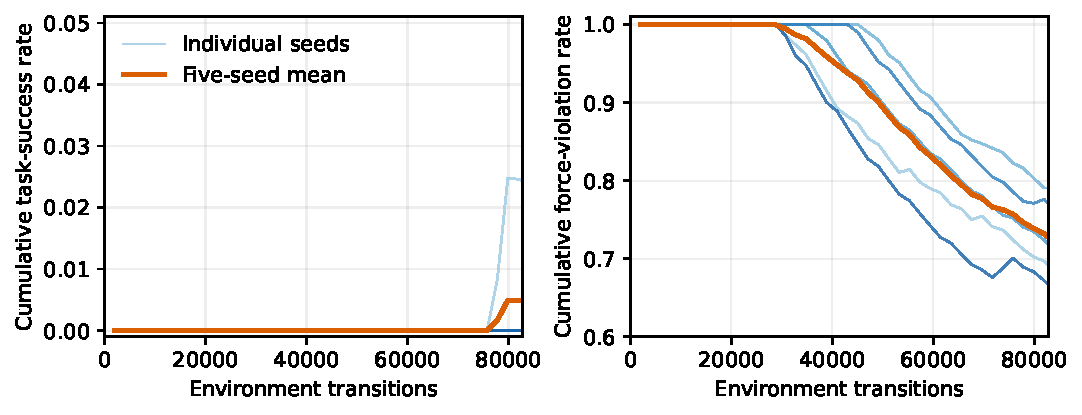
\includegraphics[width=0.92\textwidth]{figures/ppo_training_curves.pdf}
\caption{Original matched-budget direct PPO training over five seeds and
82,774 environment transitions per seed.}
\label{fig:ppo_training}
\end{figure*}

\begin{figure*}[t]
\centering
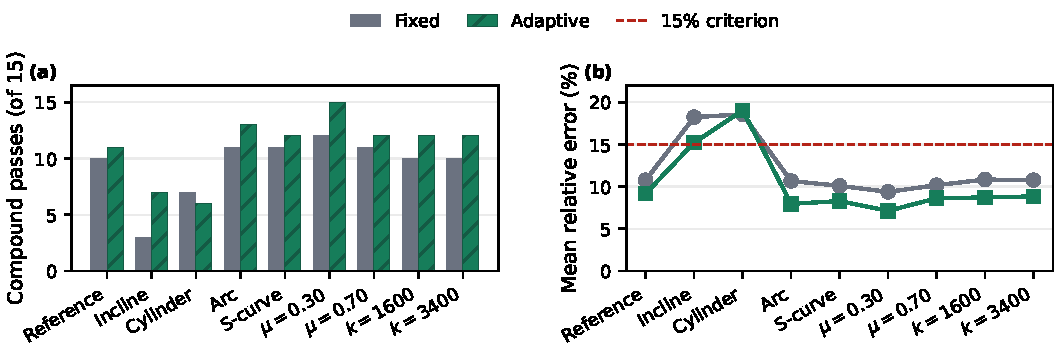
\includegraphics[width=0.96\textwidth]{figures/factor_separated_results.pdf}
\caption{Factor-separated task-and-tracking outcome and mean force error;
15 evaluations per factor level and planner.}
\label{fig:factor_results}
\end{figure*}

\section{Deployment-Gap and Cross-Engine Results}
\label{sec:deployment_gap_results}

The frozen M4 controller was evaluated in 375 new one-factor stress
evaluations.  Together with 45 reused nominal evaluations, the panel contains
420 observations over the same three blocks, five checkpoints, and three
force targets.  Every stress trace retained direct TD-MPC2 action authority;
the native simulator force remained the outcome signal while only the
learner-visible observation or registered task frame was perturbed.

\begin{table*}[t]
\centering
\caption{Severe deployment-gap endpoints. Compound counts are per 15 evaluations in each fixed block; task, tracking, and sampled-limit safety counts are over 45 evaluations. Peak force uses the native simulator signal.}
\label{tab:deployment_gap_endpoints}
\scriptsize
\begin{tabular}{lrrrrrrr}
\toprule
Condition & B0 comp. & S1 comp. & S2 comp. & Task & Tracking & Safety & Max peak (N) \\
\midrule
Nominal & 11/15 & 7/15 & 6/15 & 42/45 & 24/45 & 43/45 & 17.905 \\
Force noise 0.035~N RMS & 12/15 & 6/15 & 7/15 & 41/45 & 25/45 & 41/45 & 18.679 \\
Force bias $-0.8$~N & 14/15 & 13/15 & 4/15 & 40/45 & 31/45 & 40/45 & 22.337 \\
Force bias $+0.8$~N & 3/15 & 0/15 & 9/15 & 42/45 & 12/45 & 43/45 & 18.031 \\
Delay 50~ms & 11/15 & 12/15 & 5/15 & 34/45 & 28/45 & 35/45 & 26.084 \\
TCP error 0.10~mm & 11/15 & 7/15 & 7/15 & 44/45 & 25/45 & 44/45 & 18.491 \\
Normal error 5$^{\circ}$ & 9/15 & 8/15 & 5/15 & 30/45 & 24/45 & 41/45 & 21.316 \\
\bottomrule
\end{tabular}
\end{table*}


The signed force bias produced the clearest regulation response.  A
$+0.8$~N bias reduced compound pass from 24/45 under nominal observation to
12/45, including 11/15 to 3/15 in B0 and 7/15 to 0/15 in S1.  The corresponding
paired changes were $-53.33$ percentage points in B0 (95\% pointwise interval
$[-66.67,-40.00]$) and $-46.67$ points in S1 ($[-60.00,-33.33]$).  A
$-0.8$~N bias instead yielded 31/45 compound passes, but it also reduced task
and sampled-limit safety to 40/45 and raised the maximum native-force peak to
22.337~N.  The signed intervention therefore exposes observation bias rather
than a uniformly beneficial operating offset.

Delay and frame error affected different parts of the task.  At 50~ms,
task and sampled-limit safety fell from 42/45 and 43/45 to 34/45 and 35/45,
and the maximum peak reached 26.084~N.  A 5-degree registered-normal error
reduced task completion to 30/45 and compound pass to 22/45.  By contrast,
0.10-mm TCP-position error produced 25/45 compound passes versus 24/45
nominal, and 0.035-N RMS force noise produced 25/45.  These one-factor results
identify signed force calibration, latency, and frame alignment as the main
deployment sensitivities in the evaluated simulation blocks; their mixed
effects across B0, S1, and S2 also rule out a single monotone robustness score.

\subsection{Zero-Shot MuJoCo Stress Test}

The independently implemented MuJoCo port was evaluated only after its
open-loop mismatch had been recorded. Table~\ref{tab:cross_engine_transfer}
reports the 45 zero-shot evaluations and their matched PhysX cells. The five
frozen checkpoints achieve task completion, tracking, and sampled-limit safety
in all 30 flat and inclined evaluations. In the cylindrical block, however,
all 15 evaluations fail each component: no episode completes, every trace
exceeds 15~N, and the maximum peak reaches 20.24~N. The matched PhysX block
is also the weakest of its three surfaces, but it retains 12/15 task
successes, 6/15 tracking and compound passes, and 13/15 sampled-limit safety
passes.

\begin{table*}[t]
\centering
\caption{Zero-shot cross-engine stress results on matched checkpoint--block--target keys. Counts are out of 15 evaluations per block.}
\label{tab:cross_engine_transfer}
\scriptsize
\setlength{\tabcolsep}{5pt}
\renewcommand{\arraystretch}{0.95}
\begin{tabular}{@{}llrrrrr@{}}
\toprule
Engine & Block & Task & Tracking & Sampled safety & Compound & Max. peak (N) \\
\midrule
PhysX  & Flat reference       & 15 & 11 & 15 & 11 & 13.09 \\
MuJoCo & Flat reference       & 15 & 15 & 15 & 15 & 13.32 \\
PhysX  & $10^\circ$ incline  & 15 &  7 & 15 &  7 & 12.30 \\
MuJoCo & $10^\circ$ incline  & 15 & 15 & 15 & 15 & 13.20 \\
PhysX  & Cylinder, $r=1.2$~m & 12 &  6 & 13 &  6 & 17.90 \\
MuJoCo & Cylinder, $r=1.2$~m &  0 &  0 &  0 &  0 & 20.24 \\
\bottomrule
\end{tabular}
\end{table*}


The engine change therefore preserves the complete measured outcome on the
two planar geometries and breaks it consistently on weak curvature. Because
the calibration gate retains a bidirectional tangential-position mismatch,
this contrast is a portability stress result rather than a solver-equivalence
claim. It shows that the flat and inclined capability is not confined to one
engine implementation, while curved contact remains dependent on the policy,
geometry mapping, and contact solver as a coupled system.

\section{Provenance and Numerical Audit}
\label{sec:credibility_audit}

An independent audit re-read the 288 matched out-of-distribution traces,
verified their hashes, and recomputed all 7,776 per-evaluation metric values
without importing the experimental runner or finalizer. Every value and trace
identity matched. This verifies the reported metrics, while using the same
recorded trajectories.

The controller is time-causal but not sensor-complete. Normal force, tool pose,
and velocity come from simulator state; a registered nominal surface model
supplies the local normal and tangent used by both observation and Cartesian
action mapping. A separate binding audit verified the designated lateral and
normal impulses, but did not establish that four declared reference- or
sensor-noise labels reached the learner-visible force path. Those labels are
therefore excluded from noise-robustness claims.

The prespecified 12~N numerical panel reproduced four OOD sentinels and tested
32 paired interventions in solver iterations, contact offset, source mesh, and
their interaction. The material peak/threshold rule triggered in 11/32 cells;
task, tracking, and sampled-limit status changed in three, two, and two cells,
respectively. Ten peak responses were reductions, whereas one increase crossed
15~N. Force-tail observations consequently describe the recorded numerical
configuration rather than a general safety guarantee.

All requested source arc counts reached the mesh factory, but PhysX convex
cooking returned baseline-equivalent collision payloads in 11/12 pure mesh
cells. Only one 96-segment request changed cooked topology and triggered a
material response. The arm therefore audits request-to-collision mapping, not
multilevel mesh convergence. Detailed provenance, claim boundaries, and all
paired numerical cells are reported in the Supplementary Material.


\section{Discussion and Limitations}
\label{sec:discussion}

The factor-separated evaluation supports the proposed mechanism rather than a
simple increase in planning effort. Adaptive computation uses fewer samples,
adaptive objectives reduce force error, and their combination raises compound
pass by 11.11 percentage points with an interval that excludes zero. The
improvement is concentrated in tracking and is especially visible at 12~N,
where strict tracking rises from 5/45 to 17/45. It does not increase task
completion or reduce sampled-limit violations. High-force regulation on the
cylinder therefore remains the central performance limit.

The mechanism ablations also delimit the contribution. Moving the historical
routing threshold changes how often MPPI is used but does not expose a natural
switching point. Conversely, adding a transient-envelope head or its
target-specific calibration does not improve the frozen development outcomes.
The supported method is consequently the smaller combination of persistent
force conditioning, learned next-force risk, continuous regime-conditioned
costs, and adaptive compute allocation.

The BC ablation clarifies what \emph{direct} control requires in this study.
The evaluation controller contains no teacher or separate force regulator,
but the actor proposal is learned with behavioural supervision. Removing that
supervision leaves one-step force-model accuracy unchanged and nevertheless
eliminates contact in every development run. The result attributes BC's main
role to proposal quality for contact acquisition and recovery, not to better
force prediction. The moderate coefficient further shows that low offline
action error is insufficient: its seed-dependent failures appear only in the
closed loop.

Planning latency remains a deployment constraint. Dynamic compute reduces the
mean sample count and host planning time in the development screen, but the
simulation still runs at a 100-Hz control discretization rather than a
demonstrated 100-Hz wall-clock planner. The method should therefore be read as
a control and allocation mechanism, not as evidence of real-time execution on
the present host.

The deployment-gap panel separates several practical sensitivities.  A
0.10-mm TCP-position error and 0.035-N RMS force noise leave aggregate
compound pass close to nominal, whereas a positive force bias sharply worsens
tracking in B0 and S1.  Fifty milliseconds of observation delay reduces both
completion and sampled-limit safety, and a 5-degree registered-normal error
primarily disrupts task completion.  The opposite-signed force bias sometimes
improves the thresholded tracking count while increasing force-tail exposure,
so calibration error cannot be summarized by a single success rate.  These
isolated interventions locate deployment sensitivities without representing
a joint hardware-error distribution.

The cross-engine results separate portability from task equivalence. The
revised MuJoCo port meets the held-out multilevel normal-cycle criteria and
matches the bidirectional motion's force history, onset, and peak, but its
0.833-mm tangential-position RMSE exceeds the 0.5-mm tolerance. Zero-shot
deployment is consequently interpreted as a stress test. All 30 flat and
inclined evaluations pass, whereas all 15 cylindrical evaluations fail with
sampled-limit exceedances. The surface-specific split strengthens the
evidence for the simpler geometries, but it does not establish engine-invariant
performance. Curved contact remains sensitive to the policy, geometry
representation, and solver dynamics together.

The repeated cylinder boundary also identifies a distinct method problem.
Prior curved-surface wiping and polishing systems couple local-normal
estimation, tool-posture adaptation, and force feedback
\cite{armesto2018constraintaware,li2023unknownsurface}.
Our policy receives a registered local frame but commands translation only;
neither its latent force predictor nor its adaptive MPPI objective can rotate
the tool to follow a changing normal. A curvature-specific extension should
therefore add a bounded posture channel and compare registered, force-derived,
and learned local-normal representations under a radius sweep. Retuning the
present scalar force costs would not isolate this missing capability. We leave
that extension outside the frozen study rather than adapting the method to the
observed cylinder blocks.

The numerical audit applies unchanged. Task completion, force tracking,
contact continuity, and sampled force tails have different evidence
requirements. The final method comparison consequently reports them
separately as well as jointly. Peak force is an empirical statistic under the
recorded solver configuration. The adaptive planner's mean peak increases by
0.247~N and both planners record two samples above 15~N, so the measured
tracking benefit is not interpreted as a safety improvement. MRE and NRMSE
describe regulation on the observed contact samples.

All experiments use rigid-contact simulation and a registered nominal task
frame. The observations are causal but do not reproduce a physical camera,
force-sensor bandwidth, calibration drift, deformable contamination, or robot
communication stack. The factor-separated design improves causal
interpretation within simulation. The cross-engine stress test broadens that
evidence without replacing hardware validation.

\section{Conclusion}
\label{sec:conclusion}

This work introduced RA-RMPPI, a force-conditioned TD-MPC2 controller that
adapts both its planning objective and its computation to causal contact
regimes. Matched component studies separated objective adaptation from compute
adaptation, while behaviour-cloning, router, and risk-representation ablations
identified the smallest supported formulation. In the factor-separated
simulation study, RA-RMPPI raised compound pass from 85/135 to 100/135, reduced
MRE and NRMSE, and used fewer planning samples and less host planning time
than the fixed planner built from the same checkpoints.

The improvement is specific to force regulation and computation. Task
completion remained 132/135 versus 133/135, both planners recorded two native
samples above 15~N, and the adaptive planner had a higher mean peak force.
The cylindrical 12~N condition therefore remains a concrete boundary rather
than an exception hidden by aggregate results.  A 420-evaluation
deployment-gap panel further identified signed force bias, 50-ms delay, and
registered-normal error as distinct sensitivities. In a zero-shot MuJoCo
stress test, all 30 flat and inclined evaluations retained the compound
outcome, while all 15 weak-curvature evaluations failed; the port's remaining
tangential calibration mismatch precludes a matched-solver claim. Within the
evaluated simulation setting, the study shows that continuous regime adaptation can
make direct learned wiping more accurate and less computationally demanding,
while reliable force-tail control under curvature requires a surface-following
posture or learned-constraint extension beyond the present translation-only
action interface, followed by physical validation.


\section*{Acknowledgment}
OpenAI Codex assisted with code review, experiment automation, manuscript
organization, and language editing; the author verified all executable and
reported outputs and takes full responsibility. Code and compact results will
be released in a public Git repository, with checkpoints and traces in a
versioned archival record; stable identifiers will be inserted before
submission.

\bibliographystyle{IEEEtran}
\bibliography{PAPER_REFERENCES}

\end{document}

